\setAuthor{Jaan Kalda}
\setRound{lõppvoor}
\setYear{2007}
\setNumber{G 8}
\setDifficulty{9}
\setTopic{Geomeetriline optika}

\prob{Kuup}
\begin{wrapfigure}[16]{r}{0.5\textwidth}
	\begin{center}
		\vspace{-20pt}
		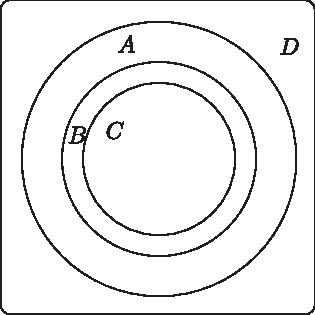
\includegraphics[width=0.95\linewidth]{2007-v3g-08-yl}
	\end{center}
\end{wrapfigure}
Läbipaistvast klaasist tehtud kuubis on suur kerakujuline õõnsus, mis on täidetud sinist värvi gaasiga. Kuup lebab kollaste seintega toas valgel põrandal. Juuresolev kuubi joonis on tehtud kuubi kohalt pildistatud foto põhjal, millelt on eemaldatud kõik värvid ning jäetud alles selgeltnähtavad kontuurid ja erivärviliste piirkondade eraldusjooned (joonte kujud ja mõõtmed on täpselt sellised nagu fotol). Kuubi mõõtmed lugeda hulga väiksemateks põranda mõõtmetest ning kõrgusest, millelt on tehtud joonise aluseks olnud foto. Millistele värvidele vastavad tähed $A$, $B$, $C$, $D$? Põhjendage vastust. Leidke klaasi murdumisnäitaja.

\hint
Kera ääres toimub pinnalt täielik sisepeegeldumine, kus peegeldunud kiired saavad alguse kas põrandalt või seinalt (ja olles seega kas valget või kollast värvi). Murdumisnäitaja määramiseks on vaja jooniselt uurida sisepeegeldumise piirjuhtu.

\solu
Välimine ringjoon on loomulikult kera välimine kontuur, tema raadius $R_A$ on võrdne kera raadiusega foto mastaabis. Kerast eemal, piirkonnas $D$, näeb läbi kuubi põrandat, st piirkond $D$ on valge. Piirkonnas $A$ toimub täielik sisepeegeldumine kera pinnal, seega näeme me sealt põranda peegeldust, mis on samuti valge. Mõõtmise teel võib veenduda, et piirkondade $A$ ja $B$ eraldusjoone raadius $R_B$ on umbes $\sqrt 2$ korda väiksem $R_A$-st, st tegemist on põranda ja seinte eraldusjoone peegeldusega. Sestap on piirkond $B$ kollane. Piirkondade $B$ ja $C$ eraldusjoon peab vastama täieliku sisepeegeldumise lõppemisele, st piirkonnas $C$ on näha kera sisemust, mis on sinine, valge põranda taustal. Niisiis on piirkond $C$ sinine. On lihtne näha, et täieliku sisepeegeldumise piirjuhul langemisnurga siinus on $\sin \alpha = R_C/R_A = 1/n$. Seega murdumisnäitaja $n = R_A/R_C \approx \num{1,8}$.
\probend